\section{Sakai Usage / \texorpdfstring{$\Delta$}{Lg} Classrank Correlation}
Grade and event data can't be joined since the event data doesn't contain a foreign key to the grade entities. However, it is worthwhile demonstrating a means by which a correlation between Sakai usage and course; such a correlation is investigated by comparing the change in class ranking of students from course results compared to admissions benchmarking scores. This value is then tested for correlation against Sakai usage for a given year, measured by presence events.

\subsection{ETL}
Using nETL, rows are extracted from the three CSV files (\textit{Admissions (2014 - 2016).csv}, \textit{Grades (2014 - 2016).csv} and \textit{Events (2016).csv}) independently of each other and concurrently, in batches of 5 000, 10 000 and 30 000 rows respectively.

Via nETL configuration, rows from the admissions data are selected for students that are South African citizens or permanents residents, and that are in undergraduate; rows from the grades data are selected for students that attended CSC1015F during 2016 and as part of their undergraduate career; rows from the events data are selected for presence events only. Dynamic filters are configured for the admissions and events data to only include students that took the CSC1015F course.

Batches of data from the CSVs is loaded into a single CouchDB database via the \textit{\_bulk\_docs} endpoint. A list of the transformations applied to each line extracted from grades / events CSV data is shown previously. The transformations applied to the events data is:

\subsubsection{nETL Events Transformations}
\begin{enumerate}
  \item A line is converted into a JavaScript object (which relates directly to the JSON format of CouchDB documents) with the fields:
        \begin{itemize}
          \item event\_date
          \item event\_id
          \item uct\_id
          \item site\_key
          \item ref
        \end{itemize}
  \item Lines are filtered on the ``uct\_id'' and ``event\_id'' fields; only events with an event type of ``presence'' (event\_id = 282) for students enrolled in CSC1015F in 2016 are considered.
  \item An attribute (``type\_'') is then added and given the value ``event'' to identify each object as a line of the Event entity type.
  \item Attributes are whitelisted. The resultant documents each have the the following attributes:
        \begin{itemize}
          \item type\_
          \item event\_date
          \item event\_id
          \item uct\_id
          \item site\_key
        \end{itemize}
\end{enumerate}

\subsection{MapReduce}
Since a single student may be associated with many rows in the Event data (sometimes even thousands of rows), a reduce function is used within the MapReduce job to aggregate the Events rows into a single document that is a count of Sakai presence events for first and second semester, with the output of this aggregation included in the index along with grade and benchmark data when reduce = true. The index consists of key:value pairs of student numbers associated a tuple that contains values for grades, benchmarks, and event information.

Each document passed to the map function is treated according to the logic shown in the activity diagram in Figure \ref{fig-3-way-join-map-function}. Logical handling of the Grade and Benchmark entities is discussed previously. If the document is a line of the Events entity then the date of the event is categorized as either having occurred in semester 1 or semester 2. A key of [Student ID, 0, Year] is emitted along with the tuple [S1, S2]. The S1, and S2 (semester) variables are 0 by default, and depending on the date of the presence event, one of these variables is altered to be `1'.

Using the \_sum reduce function, an aggregation is done across all documents with the same key; this means that per a student, an aggregation is performed on a single Grade document, a single Benchmark document, and many Events documents in which the S1 and S2 variables are summed to form the tuple [sum of S1, sum of S2]. The key emitted for each type of entity is designed so that the view-index is ordered by StudentID. For each student number, documents are ordered by the second key (course), which means that Benchmarks and Events entities are sorted to be before grades for a student; and the \nth{3} component of each key results in benchmark data always being before Events documents. As such, during view-index retrieval it can be taken as given that for a single student ID, first documents of type Benchmark will be retrieved, followed by documents of type Event, followed by documents of type Grade.

\begin{sidewaysfigure}
    \centering
    \begin{mdframed}
        \centering
        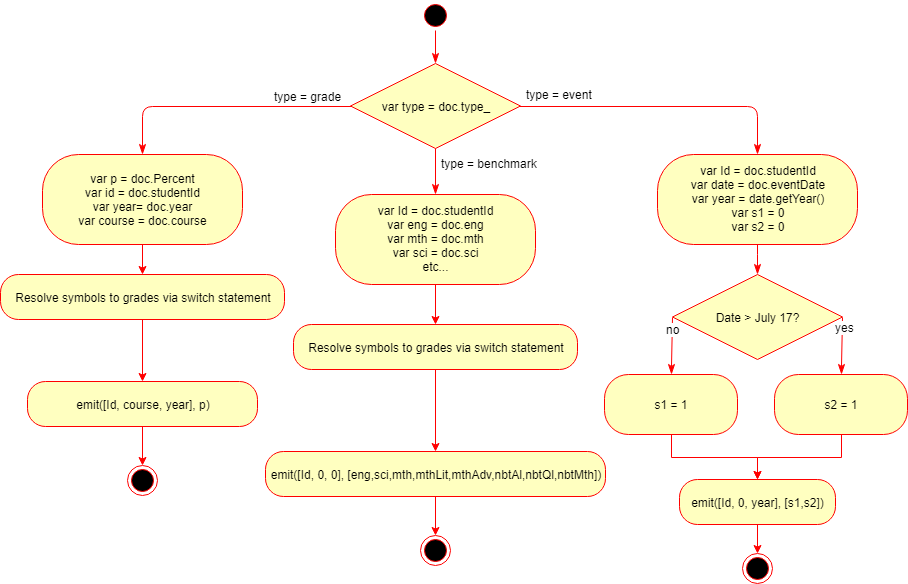
\includegraphics[scale=0.7]{./resources/figures/3-way-join-map.png}
    \end{mdframed}
    \caption[2-Way Join Map Function]{\textbf{Figure \ref{fig-3-way-join-map-function}: 3-way join \textit{map} function logic}}
    \label{fig-3-way-join-map-function}
\end{sidewaysfigure}


\subsection{List Function}
The List function is invoked via an HTTP request to the URI: \url{https://localhost:5984/msc/\_design/3-way-join/\_list/3-way-join-list/3-way-join-view?reduce=true}. On execution the list function executes the ``provides'' function, in which output type of ``CSV'' (plain text) is specified as as download file. List function logic as shown in Figure \ref{fig-3-way-join-list-function} is executed in the callback passed as a parameter to the ``provides'' function.

On initial invocation and within the body of the callback, the variables `currentStudent', `currentYear', and `currentLine' are set to null. Following this an iteration over the index is initiated with the loop control the result of a call to \mintinline{text}{getRow()} function. \mintinline{text}{getRow()} returns a row - a reduced result; in the URI the parameter ``reduce'' is set to true, so ONLY reduced output is retrieved from the view (technically, for any data sets that are not extremely small reduced output is actually the result of \textit{rereduction}). Similarly to List function logic for the 2-way join, after the loop invariant becomes false the last line is still in memory and is sent if necessary.

For every result retrieved from the reduce output , the StudentID of the row being processed is checked and compared to the StudentID of the previous row. If the current StudentID is not the same as the previous StudentID, a line of the CSV is emitted before the row is processed. Then, the type of result being processed is checked (either the document is of type ``benchmark'', ``event'' or ``grade''), and depending on the type different values are stored in a variable called ``currentLine''. For every StudentID, all types of documents are processed in turn (first the benchmark documents, then the event documents, then the grade documents) before being emitted. This allows the join to be performed via sequentially adding to the ``currentLine'' variable for a single student.

As as result of the MapReduce function, for every StudentID, exactly one ``benchmark'' result 0 or more events and one grade is processed. For every Event row processed both the first and second semester event count are exported to the CSV despite that only the first semester events are used, since there is negligible performance cost in terms of processing time or storage space and so there is little incentive to discard good data.

Sending \mintinline{text}{currentLine} is done similarly to the 2-way join except that the subroutine first checks that the currentLine variable contains data from the Grades and Benchmarks and Events entities.

\begin{figure}[H]
    \centering
    \begin{mdframed}
        \centering
        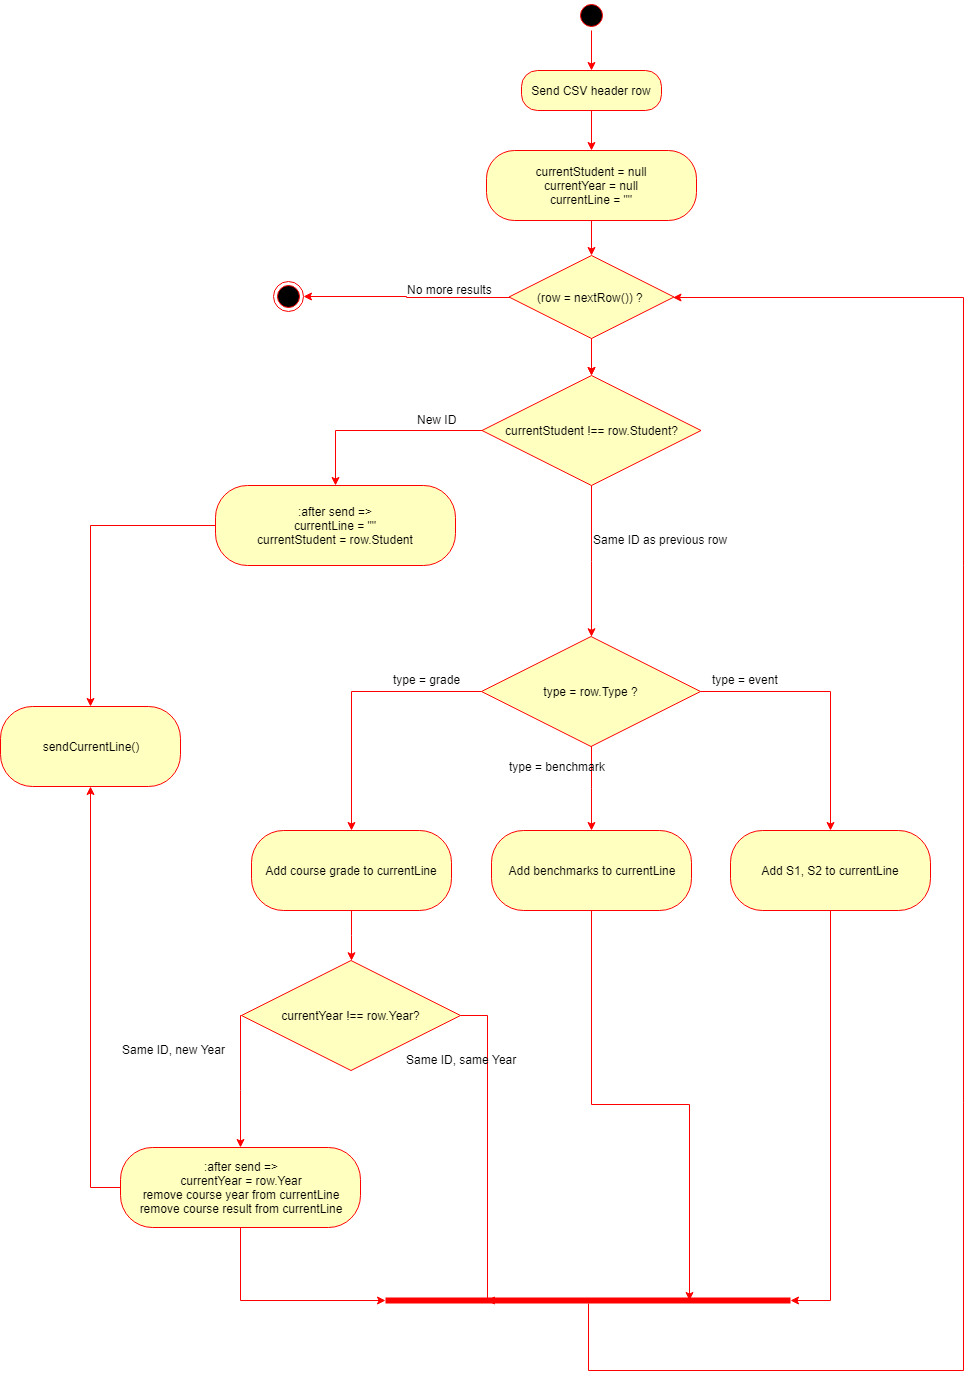
\includegraphics[scale=0.4]{./resources/figures/3-way-join-list.png}
    \end{mdframed}
    \caption[3-Way Join List Function]{\textbf{Figure \ref{fig-3-way-join-list-function}: 3-way join \textit{list} function logic}}
    \label{fig-3-way-join-list-function}
\end{figure}


\subsection{Output}
A sample of the resultant joined dataset is shown in Figure \ref{fig-3-way-csv-output}; the full CSV has 586 rows (including a header row). Since only a single year of data was analyzed, there are no repeated StudentIDs in the dataset as a student can only register for a course once per year.
\begin{sidewaysfigure}
    \centering
    \begin{mdframed}[rightline=false,leftline=false,topline=false]
        \centering
        \begin{BVerbatim}
+------+---------+----------+-------+----------+----------+----------+--------------+--------------+--------+--------+---------+------+------+
| Year |   ID    |  Course  | Grade | Gr12 Eng | Gr12 Sci | Gr12 Mth | Gr12 Mth Lit | Gr12 Mth Adv | NBT AL | NBT QL | NBT Mth |  S1  |  S2  |
+------+---------+----------+-------+----------+----------+----------+--------------+--------------+--------+--------+---------+------+------+
| 2016 | 2862568 | CSC1015F |    63 |       80 |        0 |       95 |            0 |            0 |     78 |     79 |      82 |  330 |  138 |
| 2016 | 2864266 | CSC1015F |    64 |       55 |        0 |       74 |            0 |            0 |     59 |     66 |      61 |  557 |  620 |
| 2016 | 2924430 | CSC1015F |    56 |       69 |       94 |       96 |            0 |            0 |     49 |     64 |      77 |  550 |  306 |
| 2016 | 2925212 | CSC1015F |    60 |       76 |        0 |       77 |            0 |            0 |     69 |     84 |      73 |  124 |  155 |
| 2016 | 2928032 | CSC1015F |    30 |       76 |        0 |       73 |            0 |            0 |     85 |     53 |      35 |  307 |  296 |
| 2016 | 2930116 | CSC1015F |    91 |       89 |       91 |       93 |            0 |            0 |     81 |     94 |      94 |  228 |  188 |
| 2016 | 2932174 | CSC1015F |    65 |       79 |        0 |       80 |            0 |            0 |     50 |     64 |      55 |  220 |  225 |
| 2016 | 2932204 | CSC1015F |    30 |       79 |        0 |       84 |            0 |            0 |     66 |     59 |      71 |   78 |    2 |
| 2016 | 2934500 | CSC1015F |    61 |       85 |        0 |       87 |            0 |            0 |     63 |     65 |      78 | 1054 | 1019 |
| 2016 | 2941940 | CSC1015F |    48 |       69 |        0 |       76 |            0 |            0 |     71 |     68 |      69 |  556 |  725 |
| 2016 | 2943800 | CSC1015F |    58 |       67 |        0 |       79 |            0 |            0 |     72 |     65 |      77 |  463 |  531 |
| 2016 | 2944396 | CSC1015F |    61 |       87 |        0 |       82 |            0 |            0 |     69 |     76 |      84 |  935 | 1252 |
| 2016 | 2944854 | CSC1015F |    67 |       82 |        0 |       92 |            0 |            0 |     74 |     83 |      79 |  336 |  264 |
| 2016 | 2946538 | CSC1015F |    48 |       77 |        0 |       74 |            0 |            0 |     77 |     64 |      56 |  533 |  242 |
| 2016 | 2950404 | CSC1015F |    89 |       80 |       75 |       91 |            0 |            0 |     83 |     74 |      85 |  164 |   93 |
| 2016 | 2951308 | CSC1015F |    30 |       80 |        0 |       71 |            0 |            0 |     70 |     62 |      54 |  130 |   50 |
| 2016 | 2951954 | CSC1015F |    42 |        0 |        0 |        0 |            0 |            0 |     78 |     86 |      57 |  309 |   58 |
+------+---------+----------+-------+----------+----------+----------+--------------+--------------+--------+--------+---------+------+------+
        \end{BVerbatim}
    \end{mdframed}
    \caption[Sample of 3-way CSV output]{\textbf{Figure \ref{fig-3-way-csv-output}: Sample of the 3-way join output CSV.} List function output is a CSV download with the schema as represented in this figure. The full CSV has 586 rows (including a header row). Since only a single year of data was analyzed, there are no repeated StudentIDs in the dataset.}
    \label{fig-3-way-csv-output}
\end{sidewaysfigure}
